\subsection{Cosmic Radiation Methods}
\label{sec:Minipix Testing}
	
	\subsubsection{Calibration}   
	The appropriate calibration of the MiniPIX detector was applied at The University of Houston by Dr.~Stuart P.~George, a collaborator within the Medipix Collaboration. The source calibration was applied using the \SI{60}{\keV} {\ce{^241Am} decay line, \ce{Sn} Fluorescence and \ce{^55Fe} gamma rays. The Timepix hybrid pixel detector consists of \num{65536} silicon p-n diodes, with each containing its own individual processing circuit. The response of each pixel can never be identical, thus a calibration must be performed for each individual pixel. This is a fairly complicated procedure and was our first setback. Originally, the device should have shipped with an energy calibration from the manufacturer, but we had issues with the provided energy calibration.

	The data was recorded using the Pixet Pro software provided by ADVACAM~\cite{advacam}. Dr.~George calibrated the pixel energy threshold from DAC counts to energy~\cite{stuartthesis}. The threshold was set at \SI{4}{\keV}, just above the noise level of the detector. The set threshold energy of the Timepix chip determines what energies of particles are allowed to be measured by the detector. Energy measurements in the detector are accounted by measuring the charge collected in each individual pixel. 

	\subsubsection{Collection Parameters}
        % Put the settings for the minipix shutter time, bias voltage etc. here
  	The device was configured via the device Python API wrapper provided by ADVACAM. The particle energy threshold was set to \MPThreshold, which prohibited the sensor from registering energy values that were less than the set value. Acquisition parameters were set to have a shutter time of four seconds per frame, meaning the device records four seconds' worth of data for each frame. This time was chosen as a balance between too many individual frames with little to no data, which would take up a lot of storage space, and individual frames that are so crowded with interactions that they are unreadable due to a large number of crossed tracks. Upon completing an acquisition, the device would enter a manufacturer-set dormant state for approximately two seconds, which was utilized as cool-down period to record the internal temperature of the device into a .csv file. The sensor's bias voltage was chosen to be \SI{200}{\volt} to ensure that the sensor was completely depleted. 

\subsubsection{Data Format}
The data format for each frame of data is a plain text array with each value corresponding to the time over threshold value at the corresponding pixel index in the detector. Upon the capture of a new frame the plain text array was appended to the acquisition file stored on the SD card of the RP3 on our payload. In a separate file various metadata was stored for each frame including the detector threshold, acquisition time, acquisition mode etc. The plaintext array format means that each frame of data utilized approximately 132 KB of memory. With a frame being saved roughly every six seconds, over the course of the roughly fourteen hour flight we would expect to see a total acquisition size of approximately 1.1 GB. While this is a rather small total collection size, we could have further reduced our memory footprint by only storing pixel indices with non-zero time over threshold values i.e.\ storing data in a sparse matrix format. 

%\subsubsection{Clustering Algorithm}  	
%\begin{figure}
% 	\begin{center}
% 	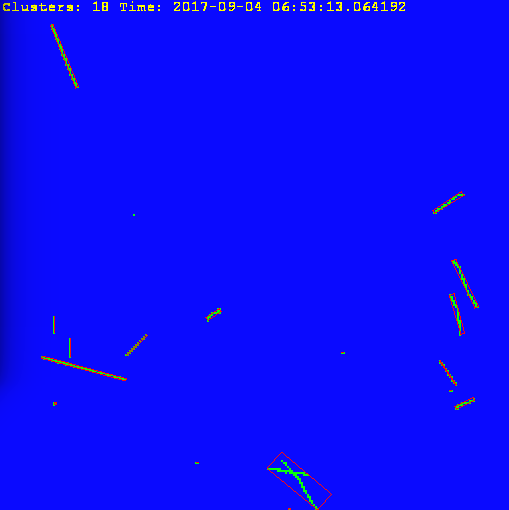
\includegraphics[width=0.5\textwidth]{./Figures/crossedtracks.png}
% 	\caption{Frame with two detector hits with crossing paths (bottom-center and shown inside red box).}
% 	\label{fig:crossedtracks}
% 	\end{center}
%\end{figure}
%
%  	Given our raw data frames after flight we needed to perform a clustering algorithm to break up each frame of data into a series of relevant parameters for each individual particle hit. It was decided that given its ease of development we would implement this algorithm in Python utilizing the Numpy scientific computing library~\cite{numpy}. While lacking the speed of C/C++, Python allowed us to quickly develop and debug the algorithm so that we could have more time to analyze the results. However, what we gained in implementation speed we lost in execution time and interactivity. Python proved to be quite slow compared to a compiled language and was rather clumsy in terms of providing interactive plots. It also took many hours each time we wanted to reanalyze our flight data. We could have avoided much of this by either writing the more processing intensive algorithms in C and creating hooks into our Python code or by simply writing the entire algorithm in C or C++.
%
%The clustering algorithm we used was a fairly straight forward flood fill implementation. We considered a cluster to be a contiguous region of pixels that registered a non-zero value. Thus, we iterated over each pixel in a frame and performed flood fill on any pixel that had not already been checked and had a non-zero value. The indices and value for each member of a contiguous region was then stored for later processing. This approach worked very well for the most part, except for when tracks from two different hits crossed, which caused two separate detector hits to be counted as one. This issue, shown in Figure~\ref{fig:crossedtracks}, occurred periodically throughout the flight but especially during ascent when cosmic ray intensity was at its peak. While this is a hard limitation of hybrid pixel detectors, a shorter frame exposure time could have prevented this issue during the high rate periods.
%
%
%
%\subsubsection{Cluster Sorting Algorithm and Morphological Analysis}
%
%Based on guidance from Dr.~George, who wrote his doctoral thesis on a hybrid pixel detector similar to the MiniPIX~\cite{stuartalgo}, we implemented a cluster sorting algorithm that sorts hits on our detector based on the pixel count, pixel density and the ratio between the length and width of the clusters bounding box. The algorithm we implemented, is nearly identical to the one developed by Dr.~George and outlined in Figure~\ref{fig:sortingalgo}. The only major difference is that, because of the thickness of the silicon chip of our MiniPIX detector, we had to increase the number of inner pixels from \num{4} to \num{8} to increase our heavy track discrimination. This is due to the fact that the original algorithm was tuned for a \SI{300}{\micro\meter} thick detector while our MiniPIX is \SI{500}{\micro\meter} thick, which resulted in thicker tracks. In general the morphological characteristics of a track left on the sensor can give us a good idea of the possible type of particle that hit the detector. For example a straight t rack on the detector is possibly explained as being deposited by a muon, fast proton or pion.
%
%	\begin{figure}[h!]
% 	\begin{center}
% 	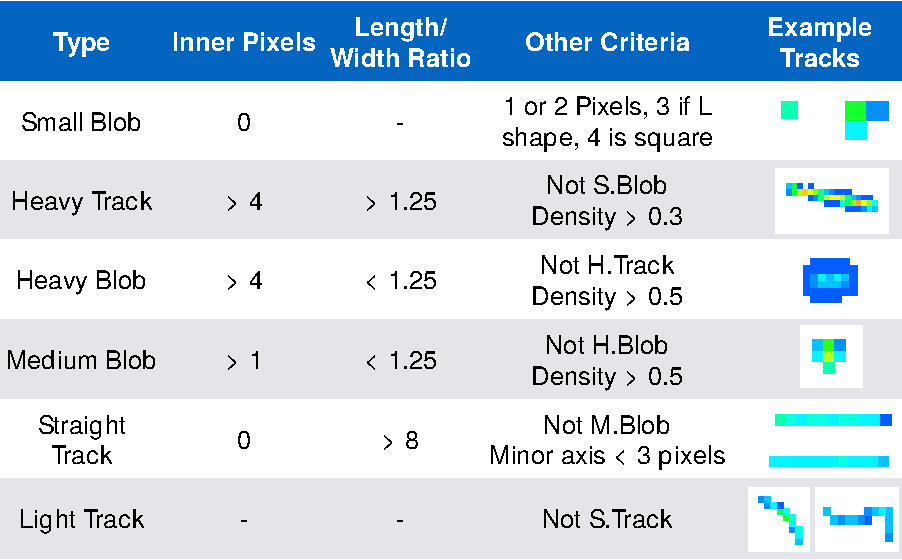
\includegraphics[width=0.75\textwidth]{./Figures/stuartgraphic.pdf}
% 	\caption{Morphological characteristics used by the sorting algorithm that is based on clusters~\cite{stuartalgo}.}
% 	\label{fig:sortingalgo}
% 	\end{center}
% 	\end{figure}
%\newpage

%\subsection{Solar Radiation Methods}
%\label{UV Photodetector Testing}

%	\subsubsection{Responsitivity and Limitations}
%	The three photodiodes used for this experiment were the JIC 139 UV photodiodes with integrated amplifiers. We used the pin configuration provided by the datasheet to create an electronic circuit to integrate the photodiodes. To filter out noise, we included a \SI{3300}{\micro\farad} capacitor for each photodiode. With this configuration, we were allowed to apply a UV light source to record the measured Voltage output $V_{\text{Out}}$ with the RESU. The photocurrent $I_{\text{PD}}$ generated from incident light on the detector can be calculated by


%	\begin{equation}
%	I_{\text{PD}} = \frac{V_{\text{Out}}}{R_{f}}
%	\label{eq:photocurrent}
%	\end{equation}


%	where $R_{f}$ is the internal feedback resistor. Then, with the calibrated specifications provided, we were allowed to determine the irradiance of UV light $E_{e}$ by
	
%	\begin{equation}
%	E_{e} = \frac{I_{PD}}{(A \cdot R)}
%	\end{equation}
	

%	where ${A}$ is the size of the active area and ${R}$ is the spectral responsitivity. The specifications and internal components that make up the photodiode determine the peak irradiance or limit of saturation where the voltage supplied (\SI{5}{\volt}) is equal to the voltage out. We used this value in Equation~(\ref{eq:photocurrent}) to calculate a maximum irradiance of \SI{189}{\milli\watt\per\square\meter} as shown in Table~\ref{tab: UV-Specs}.


%	\begin{table}[h]
%	\centering
%	\caption{Specifications and peak irradiance of the UV photodiodes.}
%	\label{tab: UV-Specs}

